\documentclass{article}
\usepackage{amsmath,amssymb}
\usepackage[numbers]{natbib}
\usepackage{geometry}
 \geometry{
 a4paper,
 total={170mm,257mm},
 left=30mm,
 top=30mm,
 right=30mm,
 bottom=30mm
 }
 
\usepackage{graphicx}
\usepackage{caption}
\usepackage{subcaption}
\usepackage{float}

\usepackage{multirow}
\usepackage{siunitx}
\usepackage{booktabs}
\usepackage{gensymb}

\usepackage{algorithm}
\usepackage{algpseudocode}

\usepackage[table]{xcolor}

\setlength{\parskip}{1em}

\newcommand{\citecustom}[1]{\citeauthor{#1} \cite{#1}}

\title{Reinforcement Learning Assignment-3 \\
	\Large Markov Decision Process and Dynamic Programming \\}
\begin{document}
\author{Utkarsh Prakash \\ \normalsize 180030042}
\maketitle
\section{Markov Decision Process}
A Markov Decision Process is a tuple $<\mathcal{S}$, $\mathcal{A}$, $\mathcal{P}$ and $\mathcal{R}>$ where $\mathcal{S}$ is the state space,
$\mathcal{A}$ is the action space, $\mathcal{P} : \mathcal{S} \times \mathcal{S} \times \mathcal{A} \rightarrow [0, 1]$ is the probability transition
function and $\mathcal{R} : \mathcal{S} \times \mathcal{S} \times \mathcal{A} \rightarrow$ $\mathbb{R}$ is the immediate reward function.
In order words, $\mathcal{P}(i, j, a) = P_{ij}(a)$ is the probability of transitioning from state $i$ to state $j$ when action $a$ is chosen.
Similarly, $\mathcal{R}(i, j, a)$ is the reward obtained on transitioning from state $i$ to state $j$ when action $a$ is chosen.

\section{Policy Iteration}
    \begin{algorithm}
        \caption{Policy Iteration}\label{policy_iteration}
        \begin{algorithmic}
            \State \textbf{input}: MDP $<\mathcal{S}$, $\mathcal{A}$, $\mathcal{P}$ and $\mathcal{R}>$, $\gamma$, $\epsilon$
            \State $\mu \gets [0,..., 0]$ \Comment{Initial Policy}
            \State $\mu^{'} \gets [0,..., 0]$ \Comment{Temporary for storing present iteration's policy}
            \While{$\mu^{'} \ne \mu$}
                \State
                \State \textbf{Policy Evaluation Step}
                \State $V^{0}_{\mu} \gets [0,..., 0]$
                \State $\delta \gets 0$
                \While{$\delta >= \epsilon$}
                    \State 1. $V^{k+1}_{\mu}(i) = \sum_{j \in \mathcal{S}} P_{ij}(\mu(i)) [\mathcal{R}(i, j, \mu(i)) + \gamma V^{k}_{\mu}(j)] \forall i \in \mathcal{S}$
                    \State 2. $\delta = \max_{i \in \mathcal{S}}(|V^{k+1}_{\mu}(i) - V^{k}_{\mu}(i)|)$
                \EndWhile
                \State 
                \State \textbf{Policy Improvement Step}
                \State The value of $V^{k+1}_{\mu}$ in the last iteration is $V_{\mu}$. Using this calculate $q_{\mu}(i, a) \forall i \in \mathcal{S}$ and $a \in \mathcal{A}$.
                \State $\mu^{'}(i) = arg \max_{a \in \mathcal{A}} q_{\mu}(i, a) \forall i \in \mathcal{S}$
            \EndWhile
            \State The policy thus obtained is the optimal policy.
        \end{algorithmic}
    \end{algorithm}

\section{Value Iteration}
\begin{algorithm}[H]
    \caption{Value Iteration}\label{value_iteration}
    \begin{algorithmic}
        \State \textbf{input}: MDP $<\mathcal{S}$, $\mathcal{A}$, $\mathcal{P}$ and $\mathcal{R}>$, $\gamma$, $\epsilon$
        \State $V^{0} \gets [0,..., 0]$
        \State $\delta \gets 0$
        \While{$\delta >= \epsilon$}
            \State 1. $V^{k+1}(i) = \max_{a \in \mathcal{A}}\sum_{j \in \mathcal{S}} P_{ij}(a) [\mathcal{R}(i, j, a) + \gamma V^{k}(j)] \forall i \in \mathcal{S}$
            \State 2. $\mu(i) = arg \max_{a \in \mathcal{A}}\sum_{j \in \mathcal{S}} P_{ij}(a) [\mathcal{R}(i, j, a) + \gamma V^{k}(j)] \forall i \in \mathcal{S}$
            \State 2. $\delta = \max_{i \in \mathcal{S}}(|V^{k+1}(i) - V^{k}(i)|)$
        \EndWhile
        \State The policy thus obtained is the optimal policy.
    \end{algorithmic}
\end{algorithm}

\section{Grid World MDP}
Let's suppose the agent lives in the $4 \times 3$ environment as shown in Table. 1. The reward that the agent gets in a particular
state is also indicated in the figure. In each of the state the agent needs to choose an action from \{Up, Down, Left, Right\}. The
agent is successful in reaching the state in which itends to reach by taking an action with probability 0.8 and reaches the states
perpendicular to the direction of action with the remaining probability (with both the perpendicular directions being equally-likely).
Let's suppose the top-leftmost cell is the origin of a coordinate system. The cell at the coordinate (2, 2) is wall or a prohibited
state. The discount factor $\gamma$ for the MDP is 0.9. 

\begin{table}[H]
    \begin{center}
    \renewcommand{\arraystretch}{2}
    \begin{tabular}{ | m{1cm} | m{1cm}| m{1cm} | m{1cm} | } 
      \hline
      0 & 0 & 0 & \cellcolor{green!25}1 \\ 
      \hline
      0 & \cellcolor{gray!25}Wall & 0 & \cellcolor{red!25}-100 \\ 
      \hline
      0 & 0 & 0 & 0 \\ 
      \hline
    \end{tabular}
    \label{grid_world}
    \caption{Grid World}
    \renewcommand{\arraystretch}{1}
\end{center}
\end{table}
	
\noindent %The next paragraph is not indented
We run the Policy iteration and Value Iteration algorithms to obtain the optimal policy and optimal value function with $\epsilon = 1e-10$.
We choose the initial policy for Policy Iteration algorithm to be moving in the Up direction for all the states. The results obtained are shown as below:

\begin{table}[H]
    \renewcommand{\arraystretch}{2}
    \begin{minipage}{.5\textwidth}
        \begin{center}
        \begin{tabular}{ | c | c| c | c | } 
            \hline
            $\rightarrow$ & $\rightarrow$ & $\rightarrow$ & \cellcolor{green!25}$\uparrow$ \\ 
            \hline
            $\uparrow$ & \cellcolor{gray!50}Wall & $\leftarrow$ & \cellcolor{red!25}$\leftarrow$ \\ 
            \hline
            $\uparrow$ & $\leftarrow$ & $\leftarrow$ & $\downarrow$ \\ 
            \hline
        \end{tabular}
        \caption{Optimal Policy}
        \end{center}
    \end{minipage}%
    \begin{minipage}{.5\textwidth}
        \begin{center}
        \begin{tabular}{ | m{1cm} | m{1cm}| m{1cm} | m{1cm} | } 
            \hline
            5.47 & 6.31 & 7.19 & \cellcolor{green!25}8.67 \\ 
            \hline
            4.80 & \cellcolor{gray!25}Wall & 3.35 & \cellcolor{red!25}-96.67 \\ 
            \hline
            4.16 & 3.65 & 3.22 & 1.52 \\ 
            \hline
        \end{tabular}
        \caption{Optimal Policy}
    \end{center}
    \end{minipage}%
    \renewcommand{\arraystretch}{1}
\end{table}

\section{Jack's Car Rental Problem}
\textbf{Example 4.2 from \citecustom{sutton2018reinforcement}}: Jack manages two locations for a nationwide car
rental company. Each day, some number of customers arrive at each location to rent cars.
If Jack has a car available, he rents it out and is credited \$10 by the national company.
If he is out of cars at that location, then the business is lost. Cars become available for
renting the day after they are returned. To help ensure that cars are available where
they are needed, Jack can move them between the two locations overnight, at a cost of
\$2 per car moved. We assume that the number of cars requested and returned at each
location are Poisson random variables, meaning that the probability that the number is
n is $\frac{\lambda^{n}}{n!}e^{-\lambda}$, where $\lambda$ is the expected number. Suppose $\lambda$ is 3 and 4 for rental requests at
the first and second locations and 3 and 2 for returns. To simplify the problem slightly,
we assume that there can be no more than 20 cars at each location (any additional cars
are returned to the nationwide company, and thus disappear from the problem) and a
maximum of five cars can be moved from one location to the other in one night. The discount factor $\gamma$ for the MDP is 0.9.\par
	
\noindent %The next paragraph is not indented 
\textbf{Time Steps:} Days \\
\textbf{Actions:} The net numbers of cars moved between the two locations overnight. \\
\textbf{States:} The state is the number of cars at each location at the end of the day. 

\subsection{Policy Iteration}
The following graphs show the sequence of policies found by the Policy Iteration algorithm starting with the policy that no car
is moved between the two locations overnight and $\epsilon=1e-4$.

\begin{figure}[H]
    \graphicspath{ {../Experiments/JackRentalProblem/PolicyIteration/} }
    \begin{center}
    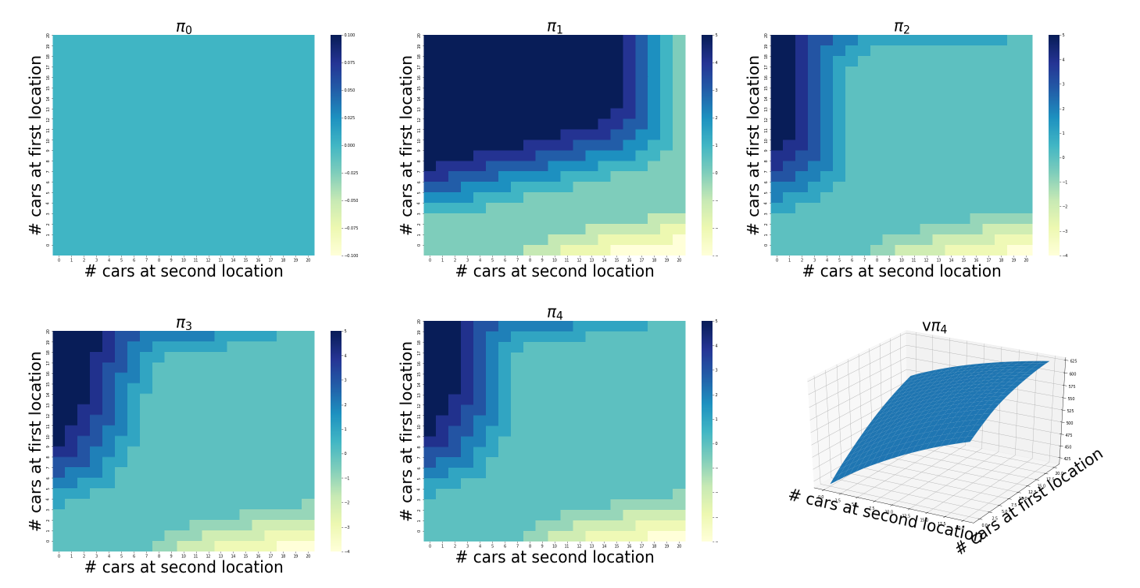
\includegraphics[width=15cm]{Compact1.png}
    \end{center}
    \caption{}
\end{figure}

\subsection{Value Iteration}



\bibliographystyle{plainnat}
\bibliography{references.bib}


\end{document}